\documentclass[jou, 11pt]{apa7}

\usepackage[american]{babel}

\usepackage{csquotes}
\usepackage[style=apa,backend=biber]{biblatex}
\addbibresource{bibliography/bibliography.bib}

\usepackage{amsmath}
\usepackage{amssymb}

\usepackage{enotez}

\usepackage[final]{microtype}

\title{The Rotation Problem}
\shorttitle{The Rotation Problem}

\authorsnames{Steven Marcel Bißantz}
\authorsaffiliations{}

\leftheader{Bißantz}

\abstract{\enquote{The Rotation problem} is an excerpt from my master thesis
\enquote{Exploratory Dimensionality Analysis in the Social Sciences -- State of
the Art and Alternative Approaches to Combat the Problem of Identifying Latent
Dimensions}. More precisely, it aims to shed light on the third of the three
major problems in exploratory factor analysis (EFA): The rotation problem.
Leaving the communality problem and the number of factor problem aside, the
excerpt focuses on (a) illuminating the topic from a researcher's perspective
while (b) developing an understanding of a more technical view on rotation --
the robot's perspective. Following the object under investigation in the social
sciences, I identify bad defaults and propose decent alternatives. This guide
will ultimately help researchers to navigate between dozens of well-known but
often poorly understood alternatives to rotate in EFA.}

\keywords{Three Major Problems, Rotation Problem, Exploratory Factor Analyis}

\authornote{
  The \LaTeX code  and the pdf-version of the writing sample are freely
  accessible on \url{https://github.com/sbissantz/smip_application}.
  For correspondence concerning the article please open an issue on Github.}

\begin{document}
\maketitle

Extracting factors using Maximum Likelihood Factor Analysis (\textsc{Mlfa})
yields--conditional on the data--the most plausible values for the above
reproduction problem. But there is usually a concern with the proposed loading
matrix. Even though the result suffices for factor-analytic robots, it is not
so for researchers. Why? Indeed, the solution describes the association between
factors and indicators; but researchers often cannot interpret it straightaway.
The loading picture is often too diffuse. Or, to put it another way, the
loading matrix has no \textit{simple
  structure}\endnote{\textcite{Thurstone1935, Thurstone1947, Thurstone1969}
  developed a set of principles on how to rearrange the loading matrix.
  Thinking in zeros and ones, one aims to redistribute both of them in the
  loading matrix to achieve an unequivocal loading pattern. At best, every item
  loads only on a single factor. If this is true for every item, the outcome
  has a simple structure: Each is attributable to (i.e., loads highly on) a
  single factor. For \textcite{Carroll1953, Tucker1955, Jennrich1966}, and
  others, this must have been a statistical fairytale. They all criticize that
  a simple structure is hardly ever reached. Nonetheless, today there are
various implementations to come close to the ideal. Some of them are part of
the following sections.}.

Transformation overcomes the problem. A transformation of the loading matrix is
visually referred to as \textsc{Rotation}. Rotations function as interpretation
aids for researchers trying to produce unambiguous loading pictures while
maintaining the extracted relationships between variables in the result. Their
outcome usually leads to a clear overall picture of the factor-item
correlations. Ultimately, rotations foster clarity by facilitating a broader
understanding of the loading pattern.

The simpler (i.\,e., more interpretable) structure can be achieved in two ways;
research can either utilize orthogonal or oblique rotation techniques. Both
will be discussed after shedding light on the researcher’s and robot’s
perspectives.

\subsection{Researcher’s perspective}

To get an idea of what it means to rotate, imagine a Cartesian coordinate
system (\autoref{fig:facord}). For ease of sake, imagine the space is
two-dimensional. With two dimensions, there are two axes $X$ and $Y$. Rename
$X$ and $Y$ using the labels of the previous \textsc{Mlfa}-result, for instance,
\enquote{honor} and \enquote{pride}. In addition, restrict the range of values
for $X$ and $Y$ to stay within the one-minus-one interval. Why minus one to
one? Because the items are now defined in terms of their loadings and loadings,
in turn, are factor-item \textit{correlations}. Let’s say the item \enquote{You
would praise a man who acts aggressively to insult} is located at
$I:(0.5,0.6)$. If the values 0.5 and 0.6 represent the item’s correlations with
each factor, one can plausible assume \enquote{You would praise a man who acts
aggressively to insult} correlates moderately to highly with \enquote{honor}
and highly with \enquote{pride}. Generalizing this logic, one can map the
entire loading matrix into the two-dimensional coordinate system. The
factor-item correlations become factor coordinates.

\begin{figure*}[htb]
\center
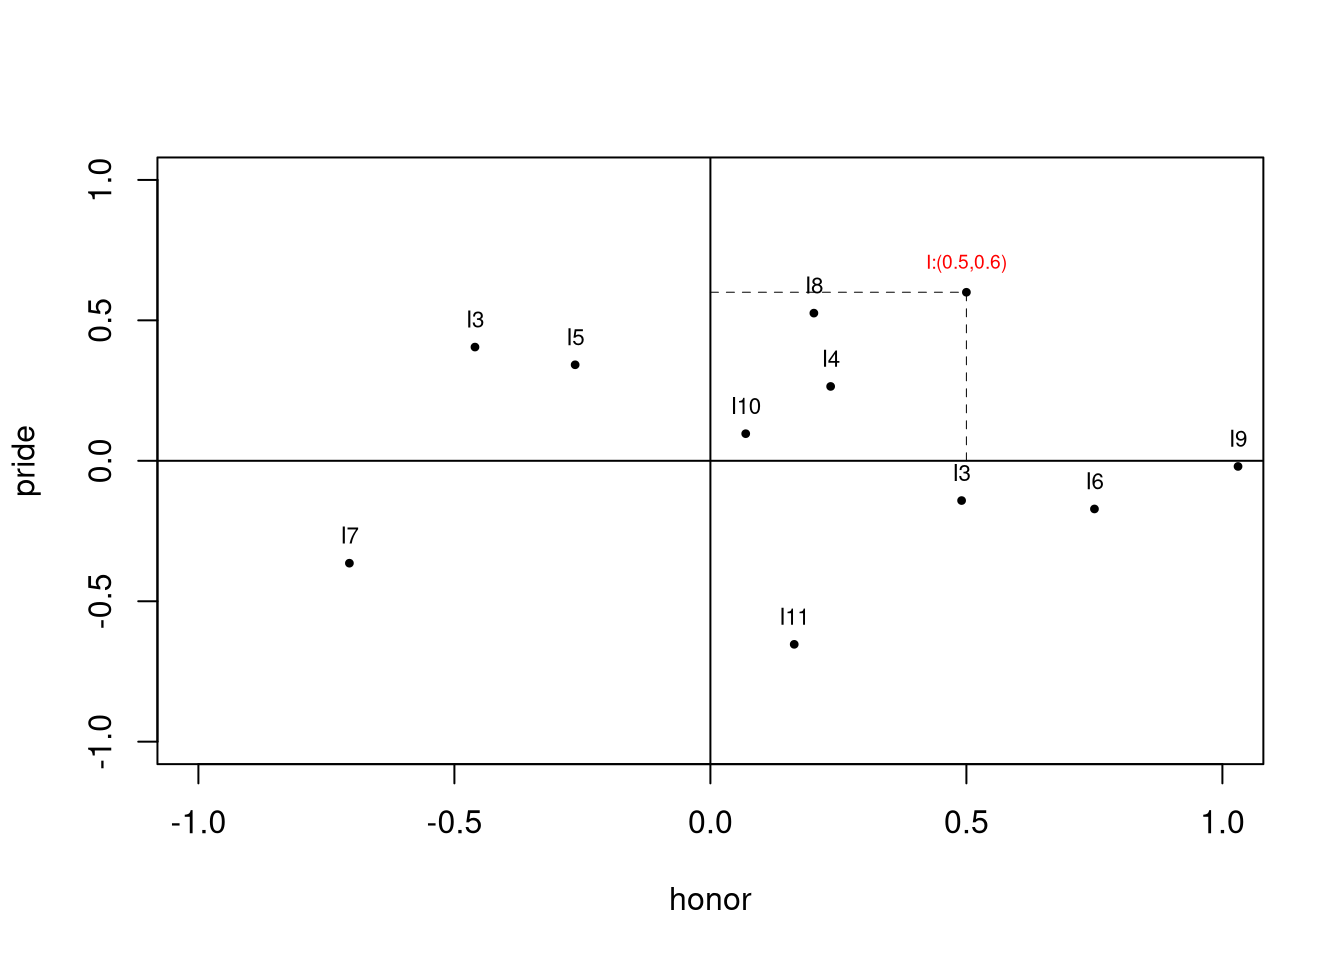
\includegraphics[scale=0.80]{figures/facord-1.png}
\caption[Factor Coordinate System]{
Factor Coordinate System -- a visualization of a loading matrix. The loadings
allow mapping the ten simulated variables in the coordinate system. The average
loading is $\bar\lambda=.55$ and the between-factor correlation is
$\phi_{12}=0.2$}
\label{fig:facord}
\end{figure*}

But does the above item, \enquote{You would praise a man who acts aggressively
to insult}, now relate to \enquote{honor} or \enquote{pride}? That is just it;
since both values are approximately equal, one cannot easily say. As mentioned
above, tackling the issue implies translating the intermediate solution into
something simple. In the graphical example, the question formulates as follows:
How to reallocate the axis in the coordinate system to generate the desired
simple(r) loading structure? The researcher has two choices: First, to
\enquote{spin the axes}, using orthogonal rotation techniques, or to apply an
oblique transformation. Both methods differ in adaptability to the object under
investigation (\textsc{Oui}) in the social sciences. While orthogonal rotations maintain
the right angle between the factor axes, transformation allows them to move
independently. The latter implies that the factors are allowed to correlate,
which will become a significant detail hereafter.

Let's pick up on understanding orthogonal and oblique techniques first. With
\textsc{Orthogonal rotation} the elementary question is how to reallocate the
axis that a simple (i.\,e., easy-to-interpret) loading-structure results. To
give an analogy, think of a spinning rotor. The rotor as a whole represents the
factor-coordinate system. The bolt (i.\,e., the origin) holds the rotor in place
so that the blades (i.\,e., the axes) can spin. When the rotor blades turn, they
maintain a fixed 90-degree angle. The same holds for factor rotation. If the
axes in a factor-coordinate system turn, the blades move counterclockwise,
preserving the right angle. Mainly, one refers to the procedure as
\enquote{orthogonal rotation}. The metaphor breaks, however, with \textsc{Oblique
rotations}. Here, one does not spin the axes, preserving the right angle between
them. The crux is to allow the axis to abandon perpendicularity explicitly.
Intuitively, one should think of the two-dimensional oblique case as a clock
(i.\,e., a factorial coordinate system) in which the hands (i.\,e., the factors)
move independently. Thus, the “time” becomes substantial (i.\,e., the angle
between the factors). It corresponds to an additional piece of information: the
between-factor correlations.

Second, the link between graphical rotation and matrix algebra should become
clear. While a visual overview is helpful to get started, it makes it difficult
to fully grasp the comprehensive modeling approach. The fact holds especially
for modern oblique techniques. To distinguish the graphical and algebraic
approach the term \textsc{Oblique transformation} \parencite{Revelle2021} will
be used. With the preliminaries set, one question remains for the following
section: What happens inside the machinery of the factorial robot? Let’s switch
perspectives to get right under the hood.

\subsection{Robot’s perspective}

From a robot’s point of view, rotation problems are a matter of solving the
transformation equation -- under different constraints. Any solution builds
upon the \textsc{Transformation equation}, formalizing as:

\begin{equation}
\hat{\Lambda}_r = \hat{\Lambda} {T}
\label{eq:transform}
\end{equation}

Notice that the equation is just a formalized version of the issue outlined
above. Namely, finding a set of axes that produces a simple(r) loading
structure ($\hat{\Lambda}_r$). More precisely, the solution just
\textit{appears} simple(r) (i.\,e., more accessible for the researcher). The
reason is that the relationships between variables are left untouched. More
technically, the robot searches a transformation matrix (${T}$) rearranging the
estimated information ($\hat{\Lambda}$) but leaving the model’s fit to the data
untouched \parencite{Mair2018}. In this light, the formal equivalent of
spinning the axis is a multiplication with this matrix (${T}$). Consequently,
the transformation matrix qualifies as the pivot point in aboves equation. It
is key to understand transformation procedures. Developing an understanding of
the transformation next will answer the question of what happens inside the
machinery.

In the orthogonal case, to multiply the plotted matrix of factor loadings
($\hat{\Lambda}$) with a transformation matrix ($T$), moves the axes
counterclockwise until the desired result ($\hat{\Lambda}_r$) is reached.
Thereby, the robot searches for a solution with two properties: Obviously, the
transformation needs to solve the transformation problem
(\autoref{eq:transform}). But even more important is the premise
of preserving the right angle between the factors. The crux is to employ a set
of orthogonal vectors because they preserve the right angle -- rotating the
factors (counterclockwise) by 90 degrees. In mathematical terms, assuming
$TT^t=I$, the orthogonalization preservation malizes as follows:

\begin{equation}
\begin{split}
  P_r & = \Lambda_r\Lambda_r^t + \Psi\\
  & = \Lambda T (\Lambda T)^t + \Psi \\ 
  & = \Lambda\underbrace{T T^t}_{I} \Lambda^t + \Psi \\
  & = \Lambda\Lambda^t + \Psi  \\ 
  & = P
\end{split}
\end{equation}

In the oblique case, solving the rotation problem implies resolving the
perpendicularity of the factor axes (algebraically, $I \neq TT^t$). Giving up
on the assumption of factor orthogonality, one literally preserves the matrix
of factor correlations ($\Phi$). The matrix of factor correlations is part of
the fundamental equation of factor analysis ($P = \Lambda \Phi \Lambda^{t} +
\Psi$) and contains the correlations between factors. For instance, if
$\Phi_{\phi_1; \phi_2} = 0.6$, where $\phi_1$ represents \enquote{honor} and
$\phi_2$ represents \enquote{pride}, the data include a high correlation
between \enquote{honor} and \enquote{pride}. Using orthogonal rotation instead,
factor-correlations are assumed to be 0, and $\Phi$ is omitted\endnote{To give
additional background, let's have a look at the pattern-structure-matrix
distinction. The structure encompasses all common information in the
correlation matrix. (1) The information between items and factors, as well as
(2) the information between factors. The decomposition is used in the
fundamental equation ($P = \Lambda \Phi \Lambda^{t} + \Psi$). If the factors do
not share any additional information, their correlation is zero ($\forall
\phi_{i,j | i \neq j} = 0$) and $\Phi$ becomes the identity matrix $I$. In this
case, the structure is reproducible using only factor-item information.
Finally, the structure (${S}$) is reproducible as a function of the factor-item
information (${\Lambda}$) and factor-factor information ($\Phi$).
Algebraically, it formalizes as: $S = \Lambda \Phi$. So rotating orthogonal
sets of the correlation between factors, the off-diagonals become zero, $\Phi$
equals $I$, and $S$ reduces to $\Lambda$. The structure matrix and pattern
matrix are identical. The key question in the following will be how realistic
the assumption of independence is in applied social science research.}.

\paragraph{Solutions}

To solve the rotation problem, researchers have two options \endnote{Since the
  pioneering work of Thurstone in the 1940s, visual rotation are also part of
  the exploratory analyzers toolkit. The problem with this rotation, however,
  is selecting factor radians. \textcite{Carroll1953}, for example, critiques
  that rotation visually induces some kind of arbitrariness in the procedure.
  Researchers are suspected of missing a concise \enquote{objective} argument
  on which to evaluate the position of the axes. As a result, researchers
  usually turn towards analytic criteria. What often remains unnoticed: Visual
  rotation allows a pretty good approximation of a simple structure
  \textcite[p. 202]{Gorsuch2015}. To combine the best of both worlds, nowadays,
analytic criteria predominate, which orient towards providing a mathematical
gateway to a simple structure}: orthogonal rotation and oblique transformation.
When it comes down to deciding on a particular one, researchers should critically
evaluate if it is reasonable to ignore the between-factor correlations. The
basis of their decision must be the correspondence with the \textsc{Oui}. Researchers
have to internalize that their decision has inevitable consequences on their
inferences. Orthogonal rotation keeps the perpendicularity of the factor axes
-- another appearance of factor independence. \textit{The decision between
  orthogonal and oblique rotations has a profound effect on the \textsc{Oui}. I
would argue that it is much stronger than selecting within the sphere of
rotation criteria}. 

To highlight the conclusion structurally, all criteria are nested regarding
their origins in the following sections (i.\,e., orthogonal rotation or oblique
transformation). Note that today, there are over two dozen rotation procedures
\parencite[pp. 214]{Gorsuch2015} -- too many to discuss them all. However,
discussing bad defaults and finding decent alternatives will be an inevitable
part of the following sections.

\subsection{Bad defaults}

Among orthogonal rotation techniques like \textsc{Quartimax}
\parencite{Carroll1953}, \textsc{Equamax} (Saunders, 1962) , and
\textsc{Orthomax} \parencite{Harman1970}; \textsc{Varimax}
\parencite[]{Kaiser1958} is the most popular choice in applied research
\parencite{Costello2005, Ford1986, Loo1979}.

\textcite{Kaiser1958}'s \textsc{Varimax} criterion proposes a solution for the
above rotation problem, maximizing the variance of the squared loadings for
each factor. This means \textsc{Varimax} is out to boost the (squared)
correlations between factors and items. In doing so, the transformation makes
the factor axis rotate by 90 degrees counterclockwise, preserving the right
angle between the factor vectors. The matrix spins the axes, so to speak.
Accordingly, Kaiser’s \textsc{Varimax} rotation subsumes under the orthogonal
rotation techniques.

But why is it a bad default? To grasp the problem, one must understand how the
orthogonality of factor-vectors relates to the assumption of independent
factors. Mathematically, they connect through the cosine. The cosine
concentrates the 360-degree spectrum to a one-minus-one range. Therefore, the
angle, a visualization of their relationship, can be transferred into a
well-known sphere of relatedness -- their correlation. As a result, if
factor-vectors are perpendicular, they should not correlate. Indeed, since
$\cos(90)$ equals 0, they do not. Thus, maintaining the 90-degree angle in
rotations preserves the right angle and consequently factor independence. There
was a cursory note on the previous finding in \textsc{Varimax}'s explanation.
\textsc{Varimax} maximizes the variance of the squared loadings. Thinking back
on the syringes in the extraction problem, \textsc{Varimax} acts accordingly; it
maximizes information density within each factor -- but at the cost of omitting
between factor correlations. Correspondingly, the result remains factor
independence.

However, there is usually no reason for the researcher to assume the
independence of factors -- especially not by default.
\textcite[p. 3]{Costello2005} urges furthermore to expect variation among
factors because \enquote{behavior is rarely partitioned into neatly packaged
units that function independently of one another}. The quote should sound
familiar, recalling the characteristic features of the \textsc{Oui} (e.\,g., its blurry
boundaries). Latent dimensions nearly always share some bits of information.
Accessing them through independent factors is a recipe for doom, inducing
ignorance bias \parencite{Loo1979}. The finding is in line with
\textcite{Sass2010}, who conducted a comparative investigation of different
rotation criteria (within the framework of exploratory factor analysis). They
encourage researchers to reflect on their rotation choices because it has a
meaningful impact on the manifestation of the factor structure. 

The habitual use of orthogonal rotations, like \textsc{Varimax}, is not
harmless. It is reasonably a bad default. It can prove a dangerous undertaking
in exploratory investigations, especially if factors demand to correlate with
each other, but chosen options hinder them in doing so \parencite{Loo1979}.
That’s the reason why switching to decent alternatives is mandatory.

\subsection{Decent alternatives}

Recall the goal of rotation and transformation procedures. They aim for
transferring the initial robot's results into something simple (i.\,e., easy to
understand). To judge simplicity among criteria, simplicity indexes come into
play \parencite[see, e.\,g.][]{Bentler1977, Kaiser1974, Lorenzo-Seva2003}.
Although they differ in terms of their mathematical formulation, conceptually
\textsc{Simplicity indexes} aim to find a solution with each item indicating
the least number of factors. In this sense, simplifying the result maximizes
interpretability.

The reason to use one of the most popular oblique transformation procedures,
like \textsc{Oblimn} and \textsc{Promax} \parencite{Hendrickson1964} is
twofold. The first argument is their correspondence with the object under
investigation (\textsc{Oui}) in the social sciences. The second is that they score high
on one of the above's simplicity criteria. It seems like a win-win situation.
On the one hand, all solutions aim to maximize factor simplicity; on the other,
they avoid factor independence. So all of them are decent alternatives. But
when it comes down to finding the most decent alternative, \textsc{Oblmin}, as
well as \textsc{Promax}, do not provide the simplest result. Indeed, they all
score high on \textit{some} indexes. But \textcite{Lorenzo-Seva2003} argues
that these are flawed ones. 

The problem is that no criteria concentrate on the loading itself. Because all
tackle the loadings merely indirectly, they miss the target, which is the
simplest loading structure doable, as a result. Bentler’s index, for example,
builds upon the \textit{colums} of the matrix of factor loadings. The loading
simplicity, in turn, focuses solely on the values of the loadings directly.

So what is the high-performance rotation criterion according to the more
accurate loading simplicity (LS) index?
\textsc{Simplimax} \parencite{Kiers1994}. In \textcite{Lorenzo-Seva2003}'s
simulation study the criterion not only outperformed more elaborate versions of
\textsc{Oblimin} and \textsc{Promax}. \textcite{Lorenzo-Seva2003} furthermore
demonstrated the \textsc{Simplimax} algorithm delivers a transformation matrix
pooling the communality of each item on the fewest number of factors. So the
rotated loading pattern is indeed as simple as possible. The factor-loadings
are either zero or as far from zero as doable \endnote{The workhorse in
\textcite{Kiers1994}'s algorithm is $\sigma(T,\Lambda_r) = || \Lambda T -
\Lambda_r ||^2$, with pattern matrix ${\Lambda}$, transformation ${T}$, and
target ${\Lambda}_r$. The crux is to find the so-called \textsc{Best simple
target}, which means to solve for a transformation (${T}$) that allows rotating
the pattern matrix ${\Lambda}$, such that the rotated matrix (${\Lambda}_r$)
has a given number ($p$) of zero entries (see: \textcite{Kiers1994} for more
details).}. 

In conclusion, \textsc{Simplimax} is the most decent alternative for two
reasons. Given the LS-index, it proved to deliver the simplest (i.\,e., most
interpretable) solution possible while keeping track of the characteristic
features of the \textsc{Oui}.

\subsection{Research recommendations}

\textit{The decision between orthogonal and oblique methods is weightier than
choosing a particular criterion}. Concerning the object under investigation,
oblique transformations prove a better standard for applied researchers. Factor
independence is an exertion rather than the rule, and oblique rotations allow
modeling factor dependencies explicitly. They permit factors to correlate with
one another while still simplifying the patterns in the loading matrix as much
as possible. Oblique transformations do no harm the \textsc{Oui}. With orthogonal
rotation, the same is not unconditionally true.

Despite their shortcoming, orthogonal rotations are a common choice in the
social sciences. Smuggling additional information into an exploratory
investigation, like factor independence, proves a profound problem in applied
research. \textcite{Loo1979} stresses this point. As one of a few, he reviewed
the (clinical) literature, questioning the appropriateness of the assumption of
independence. \textcite{Loo1979} found researchers fall back on orthogonal
rotation procedures regularly. But noteworthy is, second, in most reviewed
cases, the assumption of independence was unreasonable. Over twenty years
later, orthogonal rotations are still at the top of common-go to methods in
applied research \parencite{Ford1986, Costello2005}. It is hard to estimate how
much research is flawed by the implicit assumption of
orthogonality\endnote{\textcite{Gorsuch2015} prompts towards the rare case of
  \textcite{Guilford1981}. Replacing orthogonal with oblique transformation, he
  started reanalyzing his past research, finally resolving the assumption of
independence.}.

In this light, it is questionable to me why researchers like
\textcite{Bortz2016} are concerned with a loss in compression when going
oblique. Again, \textit{the goal in the social sciences is to compress
meaningfully, not maximally}. Although allowing the factors to correlate,
induces some redundancy; it will often prevent the researcher from having to
deal with highly distorted results \parencite{Sass2010}.

However, one should not exclude orthogonal rotations from exploratory
investigations. Previous sections suggest only to \textit{start with the least,
not the most rigid model assumption}. Learning from data implies adjusting a
model to the data, not imposing a well-known model on the data. In the rotation
or transformation context, it means to model inter-factor dependencies by
default and learn about them on the go. The conclusion is in line with
\textcite{Sass2010, Muthen1984} who recommend rotation procedures providing a
simple solution, but not at the cost of inducing incompatibility between
methods and the object under investigation. The bottom line is to find the most
simple result possible. But researchers must avoid the current practice of
finding simplicity at any cost.

Again, orthogonal rotations are not worthless in applied social-science research.
Researchers can use them strategically. For example, to highlight the added
value of resolving to assume independence. Research should become experimental,
trying different techniques and evaluating their scientific use by learning
from model differences and similarities \parencite[p. 642]{Tabachnick2007}. No
matter if results are equal across trials or completely different, in an
exploratory stage of the investigation, every finding is valuable information
about the models and how they see the data. That information should never be
excluded, suppressed, or abandoned on a preliminary ground. Researchers should
report them to improve domain knowledge.

\subsection{Additionals}

There are scenarios in which orthogonal solutions are a reasonable choice. For
example, if compressing information more fully is prior. The small additive
thus guides the application of orthogonal rotation techniques for practical
researchers. In general, \textsc{Varimax} is reasonable if factor dependence is
a minor issue or if the researcher expects more than a single general factor to
underlay a set of items \parencite[p. 195]{Gorsuch2015}. But if the researcher
anticipates a single factor, \textsc{Varimax} becomes problematic. Why? Because
it distributes the variance across factors and thus dampens the tendency of a
single factor to occur in the result \parencite{Sass2010}. As a result, if the
researcher anticipates a single general factor, \textsc{Quartimax} is the
better choice \parencite{Mair2018}. Despite that \textsc{Equamax}, combines
\textsc{Quartimax} and \textsc{Varimax}, portioning the variance more evenly
across factors \parencite[p. 214]{Gorsuch2015}. If it comes down to a single
choice for a particular criterion, \textcite{Gorsuch2015} recommends
\textsc{Varimax} because, in visual inspections, they produce interpretable
results and prove invariant across a wide range of circumstances.

The second add-on is devoted to the \textsc{Gesture of proposing}. In applied
research, dimensionality analysis is often thought of and taught as if there
has to be a definitive result. But especially in the early stages of
exploratory investigations, there might be more than one plausible solution
compatible with the constraints (e.\,g., data). In case of doubts, researchers
should start to propose different plausible solutions to the research community
\parencite[for an exception, see][]{Timmerman2017}. The conclusion is in line
with \textcite[p. 224]{Gorsuch2015} who states that any achievable result in an
early stage of theory development is an intermediate, a hypothesis, for
(follow-up) investigation yet to come. As will be shown, his suggestion holds,
especially when it comes down to determining \textit{} number of factors in the
next section.

\printendnotes 
\printbibliography

\end{document}






